\documentclass[tikz]{standalone}
\usepackage{tikz}
\usepackage[AutoFakeBold=true,AutoFakeSlant=true]{xeCJK}
\usepackage[zihao=-4,UTF8,heading=true]{ctex}
\usepackage[simplified]{pgf-umlcd}
\usetikzlibrary{positioning} %不加方向运算可能出错
\usetikzlibrary{arrows.meta} %箭头

\setCJKmainfont{微软雅黑}
\begin{document}
	\thispagestyle{empty}
    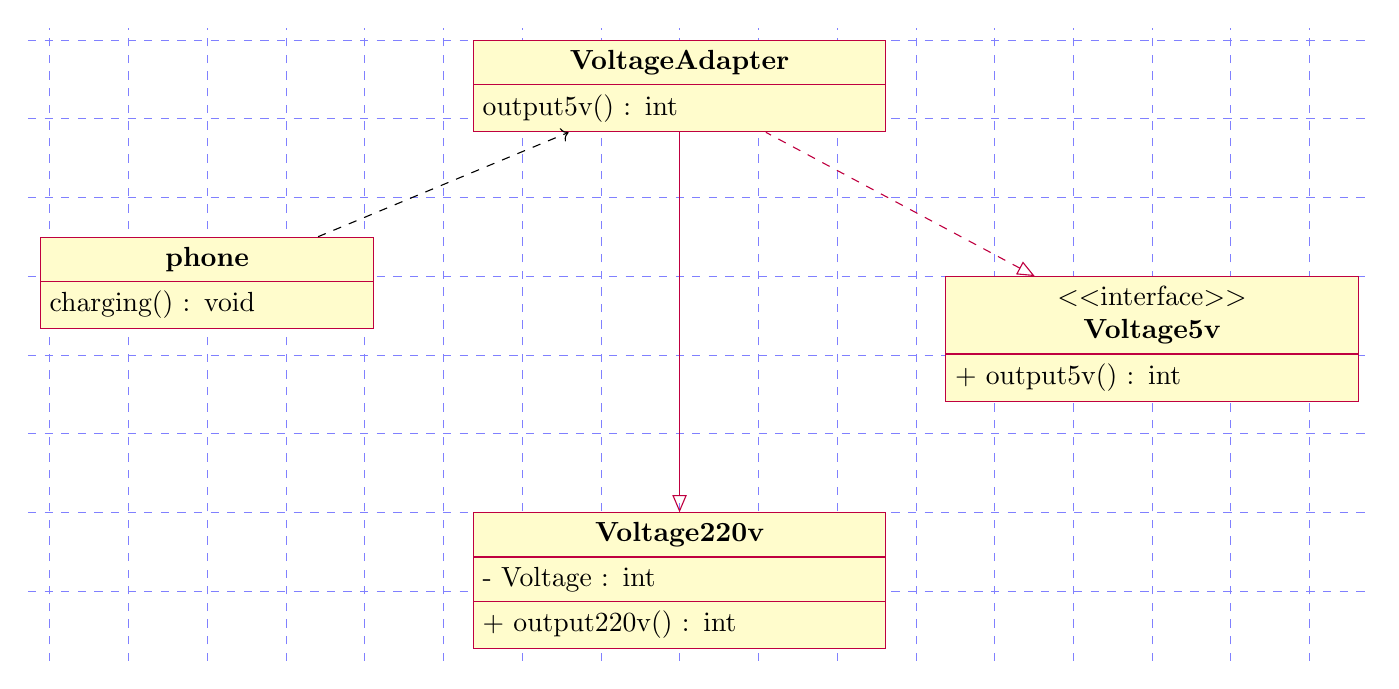
\begin{tikzpicture}[show background grid]
        \begin{class}[text width=5cm]{Voltage220v}{0,-6}
            \attribute{- Voltage : int}
            \operation{+ output220v() : int}
        \end{class}
   \begin{interface}{Voltage5v}{6,-3}
        \operation{+ output5v() : int}
   \end{interface}

    \begin{class}[text width=4cm]{phone}{-6, -2.5}
        \operation{charging() : void}
    \end{class}

    \begin{class}{VoltageAdapter}{0,0}
        \inherit{Voltage220v}
        \implement{Voltage5v}
        \operation{output5v() : int}
    \end{class}
    \draw [dashed, ->] (phone) -- (VoltageAdapter);
    \end{tikzpicture}

\end{document}